\documentclass[letterpaper,11pt,leqno]{article}
\usepackage{paper}
\usepackage{amsmath}
\usepackage{algorithm}
\usepackage{algpseudocode}
\bibliographystyle{paper}

% Local MiKTeX resolves part of the font set to bitmap (PK) fonts, which pdfTeX
% cannot font-expand; microtype's expansion then aborts the run. Protrusion (the
% larger typographic win) is unaffected. Harmless but unnecessary on Overleaf.
\microtypesetup{expansion=false}

% Float parameters. The defaults (\topfraction 0.7) forbid a top float taller
% than ~70% of the text block; both figures exceed that, so LaTeX deferred them
% and -- because the float queue is FIFO -- dragged Algorithm 1 to the end with
% them. Loosening these keeps floats near their references.
\renewcommand{\topfraction}{0.9}
\renewcommand{\bottomfraction}{0.9}
\renewcommand{\textfraction}{0.07}
\renewcommand{\floatpagefraction}{0.75}

\hypersetup{pdftitle={The Agent Is a Process: A Token-Fair Runtime for Multi-Agent LLM Systems}}

\newcommand{\bib}{paper.bib}

\begin{document}

\title{The Agent Is a Process: A Token-Fair Runtime for Multi-Agent LLM Systems}

\author{Atharva Arbat
\thanks{}}

\date{July 2026}

\paperurl{https://github.com/atharvaarbat/agent-kernel}

\begin{titlepage}
\maketitle

Multi-agent LLM systems are deployed as applications but governed as none. Concurrent agents contend for token throughput, API dollars, and provider rate-limit slots with no allocation policy beyond arrival order: a runaway agent starves its siblings, priority classes exist only in application logic, and per-agent spend is discovered after the fact on an invoice. Serving-side work has established fair scheduling \emph{inside} inference engines \citep{Sheng24}, where the quantum is a preemptible token-granular batch and the engine observes output tokens as they are produced. We address a structurally different problem one layer up, at the client runtime, where a single agent may fan out across several providers, models, and non-model tools at once. Here the quantum is an entire API call; it is non-preemptible once dispatched; and its cost is unknown until it completes. No provider can schedule this workload, because no provider sees all of it.

Our contribution is a scheduler for this regime and a proof of its fairness. Reaching it requires the right interface, so we argue that the agent is a \textbf{process}, not a chat session: the process is the abstraction under which fair scheduling is even \emph{statable}, because it supplies the per-agent budget, the scheduler state, and the single mediated boundary the scheduler operates on. We build \textbf{AgentKernel} on one invariant, \emph{complete mediation}---every model call, tool invocation, inter-agent message, clock read, and random draw passes through the kernel---and prove that no non-mediating layer, framework middleware in particular, can host the scheduler at all (Proposition~\ref{p:mediation}). On that substrate we extend virtual-time fair queueing to non-preemptible, unknown-cost quanta by charging an \emph{estimated} cost at dispatch and \emph{reconciling} the actual cost at completion. We call the discipline \textbf{Reconciled Virtual Time (RVT)} and prove a service-gap bound of $d\,(C_{\max}/w_i + \hat{E}_{\max}/w_j)$ between any two continuously backlogged agents (Theorem~\ref{t:rvt}), which specializes to $2C_{\max} + E_{\max}$ under an estimator-error parameterization (Corollary~\ref{c:estimator}) and yields starvation freedom as a corollary. Two negative results delimit the design space: without reconciliation the service gap is unbounded in time (Proposition~\ref{p:norecon}), and no non-mediating layer can enforce the premises the bound assumes (Proposition~\ref{p:mediation}). As a secondary result we adapt Dominant Resource Fairness \citep{Ghodsi11} to the agent resource vector (tokens/min, requests/min, dollars/epoch), degrading to the scalar bound when one resource dominates.

We evaluate on a deterministic mock-LLM harness driving up to 50 concurrent agents under skewed demand, adversarial bursts, and heavy-tailed output-length distributions. RVT achieves a Jain fairness index of 0.9998 (vs.\ 0.162 for FCFS and round-robin) under ${\approx}31\!:\!1$ token-cost skew ($5000\!:\!160$ tokens) at $n=10$ agents; under the primary skewed workload the observed maximum service gap is $0.67\!\times$ the Theorem~\ref{t:rvt} bound across all tested scales and five independent random seeds; and scheduling overhead is 1847\,ns per call ($<0.001\%$ of a 2\,s inference latency at $n=10$), clearing the H0a gate at both $n=10$ and $n=50$.

\end{titlepage}

\section{Introduction}\label{s:introduction}

Five agents share one API budget and one impatient human. One of them decides to summarize a two-hundred-page document and issues a 100K-token call. For the next thirty seconds the other four get nothing: the provider's rate-limit window is full, and nothing in the system is arbitrating. Whichever agent's HTTP request happened to be in flight first has won, and the human waiting on the interactive agent is paying for that accident.

This is a scheduling failure, and it is the failure this paper removes. It is worth being precise about why it persists. The dominant multi-agent frameworks---LangGraph \citep{LangChain24}, AutoGen \citep{Wu23}, CrewAI \citep{CrewAI24}, MetaGPT \citep{Hong24}, CAMEL \citep{Li23}---are orchestration libraries. They define \emph{what} agents say to each other: the graph, the handoff protocol, the role prompts. None of them defines \emph{how the system's scarce resources are allocated} when those agents run at the same time. The result is a class of systems that have concurrency without a concurrency policy.

\subsection{The deficit}\label{s:deficit}

Three symptoms recur across deployments.

\textbf{Monopolization.} A single agent issuing large or frequent calls saturates the provider's rate-limit window and stalls every sibling for the remainder of the epoch. There is no notion of a share, so there is no notion of exceeding one.

\textbf{Unenforced priority.} Applications routinely distinguish a user-facing agent from a background one, but the distinction lives in comments and naming conventions. Nothing at the infrastructure layer dispatches the interactive agent first, and nothing prevents the background agent from consuming the window.

\textbf{Retroactive accounting.} Dollar spend is metered by the provider after the fact. No runtime enforces a per-agent budget, so a looping agent's cost is discovered when the bill arrives rather than when the loop starts.

The resource vector is itself unusual. Agents contend simultaneously over \emph{tokens per minute} (the provider's throughput limit), \emph{requests per minute} (a separate concurrency limit), and \emph{dollars per epoch} (a cost budget). These dimensions are not proportional to one another. An agent issuing many short calls bottlenecks on requests/min while an agent issuing a few long ones bottlenecks on tokens/min; a third, calling an expensive reasoning model rarely, bottlenecks on dollars. Scalar fair share is not merely hard to compute in this setting---it is ill-defined, because the agents are not competing for the same scalar.

\subsection{Why the runtime is the right vantage point}\label{s:vantage}

One could ask the providers to be fair, and for a single model behind a single API, VTC \citep{Sheng24} shows how. But an agent system is not a single model behind a single API. In a realistic deployment, Agent~A reasons with GPT-4 while Agent~B reasons with Claude; Agent~C's spend is dominated by a web-search tool and Agent~D's by a database it queries repeatedly, so that for those two the model calls are a minority of the cost; and all four share one session budget in dollars and one human's patience in latency.

No provider can see this picture. OpenAI's scheduler sees Agent~A's calls and nothing of B, C, D, the search tool, or the database. Anthropic's scheduler sees the mirror image. The search API sees neither. \textbf{The only vantage point from which the whole resource contention is visible is the runtime the agents share.} Fairness, budgets, and priority are therefore properties that can only be enforced \emph{above} the provider, across heterogeneous back-ends, and over both model and non-model resources.

Figure~\ref{f:mediation} makes the vantage point literal. Every back-end---two providers and two external tools---crosses one boundary, and only the runtime that owns that boundary sees them all at once. This is what makes client-side scheduling a distinct and necessary problem rather than a redundant copy of serving-side scheduling.

\begin{figure}[tbp]
\centering
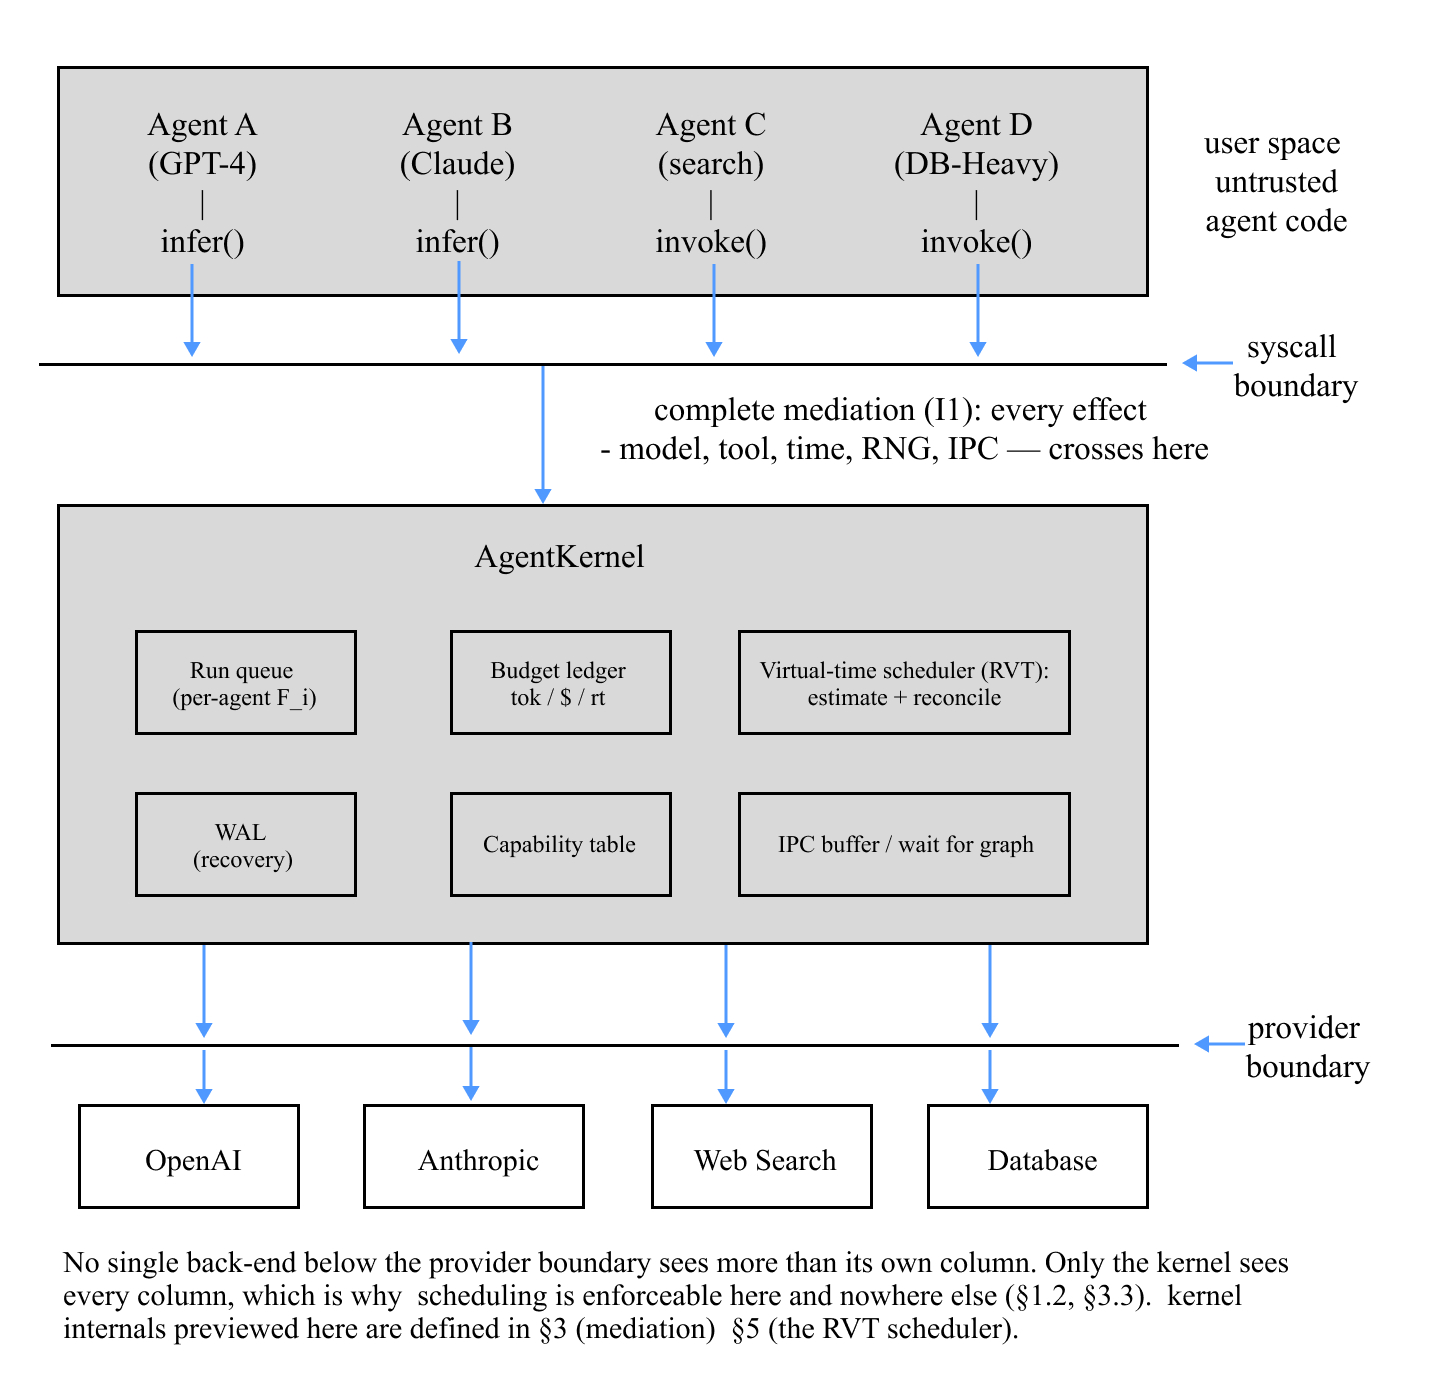
\includegraphics[width=0.85\textwidth]{figures/figure_1.jpg}
\caption{The complete-mediation boundary. Four agents, each with a different dominant back-end, issue \texttt{infer} and \texttt{invoke} syscalls that cross a single boundary into AgentKernel; the kernel's run queue, budget ledger, virtual-time scheduler, write-ahead log, capability table, and IPC buffer sit above a second boundary, below which each provider or tool sees only its own column. No back-end below the provider boundary sees more than one column; only the kernel sees every column, which is why fair scheduling is enforceable here and nowhere else (\S\ref{s:vantage}, \S\ref{s:mediation}).}
\label{f:mediation}
\end{figure}

\subsection{Why existing scheduling theory does not transfer}\label{s:theorygap}

VTC \citep{Sheng24} proves a $2\times$ service bound for LLM serving and is the closest prior work. It operates inside the serving engine, where continuous batching \citep{Yu22} permits preemption at token granularity and the engine observes output tokens as they are generated. At the client runtime, three properties invert.

\emph{The quantum is an entire call.} Once dispatched, an \texttt{infer} cannot be preempted mid-token. The scheduler's only mid-call primitive is \texttt{cancel}, which truncates and forfeits the work done so far.

\emph{Cost is unknown at dispatch.} The scheduler must commit to a dispatch order before knowing how long the call will run or how much it will cost, because output length---the dominant cost term---is revealed only on completion.

\emph{The scheduler is above the provider API.} It cannot interpose on token generation to reclaim the resource early, and it cannot see the queueing that happens on the far side of the boundary.

This is closer to packet scheduling with unknown packet sizes over a constrained link---a regime classical fair queueing explicitly excludes, since WFQ \citep{Demers89} and SFQ \citep{Goyal96} both assume the packet size is known at enqueue, as do lottery and stride scheduling \citep{Waldspurger94, Waldspurger95}. Worse, unlike a router, we cannot drop or fragment. A fairness bound for this regime must account for both the non-preemptibility gap---one long call holding the resource past its fair quota---and the error introduced by predicting cost. Neither VTC's analysis nor the classical fair-queueing analyses cover it.

\subsection{Thesis}\label{s:thesis}

\begin{quote}
The process abstraction, not the chat abstraction, is the correct systems interface for autonomous LLM execution. An LLM agent is a process: it has a private context region, a resource budget, scheduler state, message channels, and a lifecycle. If a runtime enforces complete mediation---the agent never touches the model, tools, time, randomness, or other agents except through the kernel---then proportional-share scheduling becomes implementable with classical virtual-time machinery, adapted for non-preemptible, unknown-cost quanta.
\end{quote}

Complete mediation is not merely convenient for this; \S\ref{s:mediation} proves it necessary. The scheduler that results, Reconciled Virtual Time, is the paper's central result. The process abstraction earns its place in the paper by being what makes that result statable and provable.

\subsection{Contributions}\label{s:contributions}

\begin{enumerate}
\item \textbf{Reconciled Virtual Time (RVT)} (\S\ref{s:rvt}): a proportional-share discipline for non-preemptible, cost-unknown-until-completion quanta, with a proven service-gap bound (Theorem~\ref{t:rvt}), starvation freedom (Corollary~\ref{c:starvation}), and a matching lower bound (Proposition~\ref{p:tightness}). The analysis isolates \emph{reconciliation} as the mechanism that bounds unfairness and shows that the estimator affects the bound only through the magnitude of the in-flight charge, not through its accuracy---a result that revises the intuition that better prediction buys fairness.
\item \textbf{Two negative results} delimiting the design space: without reconciliation the service gap grows without bound in time (Proposition~\ref{p:norecon}), and no non-mediating layer---framework middleware in particular---can enforce the premises the bound requires (Proposition~\ref{p:mediation}).
\item \textbf{The agent-process abstraction that makes RVT statable} (\S\ref{s:process}): a field-by-field process control block for agents, a fixed syscall surface, five invariants, and a stratification of execution forms by how completely each closes the bypasses Proposition~\ref{p:mediation} enumerates.
\item \textbf{An implemented runtime and evaluation harness} (\S\ref{s:implementation}, \S\ref{s:evaluation}): AgentKernel---syscall interface, budget ledger, write-ahead log, and two enforced execution forms---together with a deterministic mock-LLM harness and an adversarial workload suite. The harness validates H0a (scheduling overhead), H1a (Jain fairness under cost skew), and H1b (Theorem~\ref{t:rvt} service-gap bound). Starvation freedom is established as Corollary~\ref{c:starvation}, a direct theorem consequence rather than a simulation result. DRF multi-resource fairness (\S\ref{s:drf}) and the mediation-leakage escape suite (Proposition~\ref{p:mediation}) are secondary results with empirical validation deferred to future work.
\end{enumerate}

\section{Problem Statement and System Model}\label{s:model}

We fix notation used throughout.

\textbf{Agents and weights.} A set of agent processes $i = 1 \ldots n$ share one kernel. Agent $i$ carries a positive weight $w_i$ expressing its entitled share; equal weights give equal shares. Weights are administrative input, not inferred from behavior.

\textbf{Calls and cost.} Agent $i$ submits calls $c$ through the syscall interface (\S\ref{s:syscall}). Following the VTC cost form \citep{Sheng24}, an \texttt{infer} call has cost
\[
  \mathrm{cost}(c) \;=\; \alpha \cdot \mathrm{in\_tokens}(c) \;+\; \beta \cdot \mathrm{out\_tokens}(c),
\]
where $\alpha, \beta > 0$ are provider- and model-specific coefficients. Non-model \texttt{invoke} calls carry a cost in the same units, either metered by the tool or assigned by policy. We write $a(c)$ for the \emph{actual} cost, revealed only at completion, and $\hat{e}(c)$ for the kernel's \emph{estimate}, computed at dispatch. Crucially, $\mathrm{in\_tokens}(c)$ is known at dispatch and $\mathrm{out\_tokens}(c)$ is not, so the uncertainty is confined to the $\beta$ term but is not thereby small: output length is the heavy-tailed component.

\textbf{Non-preemptibility.} Once a call is dispatched to a provider it runs to completion. The only intervention available is \texttt{cancel}, which truncates the call; the tokens already generated are still charged, so cancellation forfeits work rather than reclaiming it.

\textbf{Concurrency.} The kernel dispatches from a single logical loop, so dispatch decisions are totally ordered (this also makes them loggable and deterministic; \S\ref{s:invariants}, I4). Each agent may have at most $d$ calls in flight simultaneously, a kernel-configured bound. The natural setting for a sequential agent is $d = 1$: the agent blocks on its \texttt{infer} and cannot issue another until it returns. Fan-out agents run with $d > 1$.

\textbf{Constraints.} Dispatch is subject to provider-side admission constraints---requests per minute, tokens per minute---and to per-agent budget constraints in tokens and dollars. We write $\mathrm{admissible}(i)$ for the predicate that agent $i$'s next call may be issued now without violating either.

\textbf{Service.} Define $A_i(t)$, the \emph{reconciled service} of agent $i$, as the sum of actual costs $a(c)$ over all of $i$'s calls completed by time $t$. This is the quantity fairness is about: what the agent actually consumed, not what it was predicted to consume.

\textbf{Objectives.} The scheduler must be (a) \emph{fair}: bound $|A_i(t)/w_i - A_j(t)/w_j|$ for continuously backlogged $i, j$; (b) \emph{starvation-free}: every backlogged agent is dispatched within bounded work, including under priority classes; (c) \emph{work-conserving}: never idle while some backlogged agent is admissible; and (d) \emph{deterministic}: given the log prefix, the dispatch sequence is a function of logged state.

\textbf{Bounded quantities.} We assume $a(c) \le C_{\max}$ and $\hat{e}(c) \le \hat{E}_{\max}$ for all calls, and $a(c) \ge c_{\min} > 0$. The first holds because providers cap \texttt{max\_tokens}; the second because the kernel controls the estimator; the third because every call consumes at least its prompt.

\section{The Agent-Process Abstraction}\label{s:process}

The title claims an agent is a process. This section discharges that claim: it reconstructs the process control block for an agent (\S\ref{s:pcb}), defines the syscall interface that gives the abstraction teeth (\S\ref{s:syscall}), proves that only a mediating kernel can host it (\S\ref{s:mediation}), states the invariants the kernel enforces (\S\ref{s:invariants}), and stratifies the execution forms by the assurance each provides (\S\ref{s:forms}). We build the abstraction here not for its own sake but because \S\ref{s:rvt}'s scheduler cannot be \emph{stated} without it: the budget vector, the per-agent scheduler state, and the single mediated boundary are precisely the preconditions Theorem~\ref{t:rvt} assumes.

\subsection{The process, reconstructed}\label{s:pcb}

A classical process is not its code; it is the kernel's bookkeeping \emph{about} that code---the process control block. An agent admits the same bookkeeping, field for field. The correspondence below is not an analogy for rhetorical effect: each row names a concrete data structure the kernel maintains and the concrete mechanism it enables.

\begin{table}[t]
\caption{Classical PCB fields and their agent-process analogues}
\label{t:pcb}
\begin{tabular*}{\textwidth}{p{3.5cm}@{\extracolsep\fill}p{5cm}p{4.5cm}}
\toprule
Classical PCB field & Agent-process analogue & Enables \\
\midrule
Address space / page tables & Context region $C$ (per-agent working set) & Isolation of one agent's working set from another's \\
Registers / program counter & Conversation state + pending tool calls & Resumption after a blocking syscall \\
Scheduler state (nice, vruntime) & Virtual time $F_i$, weight $w_i$, priority $\pi$ & Proportional-share dispatch (\S\ref{s:rvt}) \\
Resource limits (\texttt{rlimit}) & Budget vector $B = (B_{\mathrm{tok}}, B_{\$}, B_{\mathrm{rate}})$ & Per-agent budget enforcement \\
File descriptor table & Tool handles / capabilities & Least-authority tool access \\
Signals & \texttt{cancel} (preemption by truncation) & The only mid-call preemption primitive available \\
IPC (pipes, message queues) & \texttt{send}/\texttt{recv} + kernel message buffer & Inter-agent coordination the kernel can observe \\
Process state \{\hbox{run, ready, blocked}\} & \{\texttt{created, runnable, running, blocked, terminated}\} & Lifecycle accounting; wait-for graph \\
\bottomrule
\end{tabular*}
\end{table}

\begin{definition}[Agent process]\label{d:agent}
An agent process is a tuple $P = (\mathit{id}, S, C, B, \pi, L)$ where $S \in \{\texttt{created}, \texttt{runnable}, \texttt{running}, \texttt{blocked}, \texttt{terminated}\}$ is the lifecycle state; $C$ is the private context region; $B = (B_{\mathrm{tok}}, B_{\$}, B_{\mathrm{rate}})$ is the multi-resource budget vector; $\pi$ is the priority class; and $L$ is the handle into the write-ahead log.
\end{definition}

The single structural difference from a UNIX process is the one that generates this paper's entire technical contribution. \textbf{A classical scheduler knows the cost of the quantum it is about to run---one timeslice---and can reclaim the CPU at the end of it with a timer interrupt. The agent scheduler knows neither: the cost of an \texttt{infer} is unknown until it returns, and no interrupt can reclaim a call in flight.} Section~\ref{s:rvt} is the repair of that one break.

\subsection{The syscall interface}\label{s:syscall}

The abstraction is real only if the agent cannot act except through it. The kernel exposes a small, fixed syscall surface---the only channel between an agent and the world:

\texttt{infer} (model call), \texttt{cancel} (abort an in-flight call), \texttt{invoke} (tool call), \texttt{send}/\texttt{recv} (inter-agent messages), \texttt{clock}, \texttt{random}, \texttt{spawn}, \texttt{exit}.

Every syscall is scheduled and logged. Each tool handle passed to \texttt{invoke} is an explicit capability rather than an ambient permission (\S\ref{s:invariants}, I2); this paper relies on that only insofar as the scheduler must attribute every tool call to an agent, and leaves capability enforcement and its security analysis out of scope. \texttt{send} is asynchronous and kernel-buffered; \texttt{recv} blocks, moving the agent to \texttt{blocked}. Because the kernel observes every \texttt{recv} wait, it maintains the inter-agent wait-for graph, which is what makes deadlock detection and cross-agent priority inheritance possible (\S\ref{s:priorities})---a scheduling dividend of mediation rather than a separate subsystem.

Figure~\ref{f:mediation} shows this surface concretely: every agent arrow terminates at the syscall boundary, and nothing reaches a provider except through the kernel sitting on it.

\subsection{Why a kernel, and not middleware}\label{s:mediation}

A reviewer will reasonably ask why the scheduler needs a privileged kernel rather than cooperative middleware: a framework could intercept LLM-client calls as a library shim. The answer is that the scheduler depends on properties a non-mediating layer cannot supply. We state this as a proposition not because the conclusion is mathematically surprising---given the definitions of P1--P3, the proof is nearly immediate for each case---but because the value is in the enumeration: it names exactly which channels must be mediated and which scheduler guarantee each unmediated channel defeats, giving the architecture decision a precise technical warrant rather than a design opinion.

\begin{proposition}[Necessity of complete mediation]\label{p:mediation}
Let a scheduler require, for its fairness and starvation guarantees, that (P1) every resource-consuming effect is \emph{charged} to an agent before it takes effect; (P2) effects are \emph{serialized} through a single dispatch decision the scheduler controls; and (P3) every inter-agent wait is \emph{observable} to the scheduler. Then any layer $M$ that does not mediate all of $\{\texttt{infer}, \texttt{invoke}, \texttt{send}/\texttt{recv}, \texttt{clock}, \texttt{random}\}$ cannot guarantee P1--P3.
\end{proposition}

\begin{proof}
Suppose $M$ leaves some syscall unmediated. We show each case defeats at least one required property.

\emph{Clock.} If $M$ does not mediate \texttt{clock}, an agent reads wall-clock time directly and can busy-wait, poll, or time its own bursts outside the scheduler's frame. The scheduler cannot serialize activity it never observes, defeating P2.

\emph{Model and tool calls.} If $M$ does not mediate every \texttt{infer} and \texttt{invoke}, an agent can construct a model or tool client directly---a raw socket, a second SDK instance---and consume tokens and dollars never charged to the ledger. The sum of charged costs then diverges from metered usage, defeating P1 (and with it invariant I5, on which Theorem~\ref{t:rvt}'s identification of $A_i$ with real consumption depends).

\emph{IPC.} If $M$ does not mediate \texttt{send}/\texttt{recv}, agents coordinate through a side channel---a shared file, an external message bus---and block on one another invisibly. The wait-for graph is then incomplete, so priority inheritance and deadlock detection are unsound, defeating P3.

\emph{Ordering.} If any effect reaches a provider without passing the dispatch point, the scheduler's serialization is advisory rather than enforced: a backlogged agent jumps the queue simply by not calling the mediated path, defeating P2.

\emph{Randomness.} If $M$ does not mediate \texttt{random}, agent behavior---including retry and backoff timing, which consumes rate-limit slots---is neither reproducible nor accountable, so the scheduler cannot bound the contention it is meant to control.

Each bypass is available to any layer that agents can go \emph{around}. A layer can be gone around exactly when it does not sit on the sole path to the effect---that is, when it is not a mediating kernel. Hence complete mediation over $\{\texttt{infer}, \texttt{invoke}, \texttt{send}/\texttt{recv}, \texttt{clock}, \texttt{random}\}$ is necessary for P1--P3.
\end{proof}

The corollary is architectural: middleware can \emph{approximate} the scheduler but cannot \emph{guarantee} it, because an agent---or a bug---can always construct the underlying client itself. This is why \S\ref{s:forms} stratifies execution forms by how strongly each closes the bypasses; measuring shim leakage empirically is the work of the escape suite described in \S\ref{s:limitations} and left to future evaluation.

\subsection{Invariants}\label{s:invariants}

The kernel enforces five invariants. This paper proves the scheduling consequences of I1, I4, and I5; I2 and I3 are part of the kernel's design and are stated here to fix the interface, but their security and recovery implications are beyond a scheduling paper's scope.

\begin{description}
\item[I1 (complete mediation \citep{Saltzer75}).] No agent-visible or agent-external effect occurs except via a syscall. Proposition~\ref{p:mediation} shows I1 is necessary for the scheduler's guarantees; \S\ref{s:rvt} shows it is sufficient.
\item[I2 (no ambient authority \citep{Dennis66, Miller06}).] Every \texttt{invoke} carries an explicit capability rather than relying on the agent's ambient permissions. The scheduler uses this only to attribute each tool call to an agent.
\item[I3 (log-before-effect \citep{Mohan92}).] Every nondeterministic input is durably appended to the write-ahead log before the agent observes it. Here the log serves crash recovery; we do not exploit it for deterministic replay.
\item[I4 (deterministic kernel).] Given the log prefix, every kernel decision is a deterministic function of logged state. This constrains the scheduler concretely: ties in $F_i$ must be broken deterministically, and the dispatch order is itself a logged event.
\item[I5 (budget conservation).] Ledger accounting is exact: the sum of per-agent charged costs equals metered provider usage within reconciliation error. Theorem~\ref{t:rvt} bounds a gap in \emph{charged} service; I5 is what makes that a statement about real consumption.
\end{description}

\subsection{Enforcing I1: agent execution forms}\label{s:forms}

I1 is a claim about what agent code \emph{cannot} do, so it is only as strong as the environment hosting that code. Classical kernels get user/kernel separation from a hardware privilege bit; we must buy it. AgentKernel defines two supported forms, ordered by how completely they close the Proposition~\ref{p:mediation} bypasses.

\textbf{SDK agents (cooperative mediation).} Agents are written against the kernel's syscall SDK; mediation is by convention plus static lint that rejects network, clock, and RNG imports in agent packages. Assurance is ``the developer did not bypass''---sufficient for the scheduling and budget-conservation claims, insufficient against agent code that deliberately bypasses the SDK.

\textbf{Sandboxed agents (enforced mediation).} Agent code runs in a WASM module \citep{Haas17} or an OS process in a network-denied namespace, whose only host imports are the kernel syscall shims. Here I1 holds by construction against arbitrary agent code: the bypasses are physically unavailable.

For existing framework code, a \textbf{compatibility shim} intercepts the LLM- and tool-client call surface and reroutes those calls as syscalls. It is a migration path, not a guarantee; by Proposition~\ref{p:mediation} it is exactly the leaky case, measuring its leakage with an adversarial escape suite and reporting which invariants survive is future work (\S\ref{s:limitations}).

\section{Reconciled Virtual Time}\label{s:rvt}

We develop the scheduler the way a reader meets the problem: start from the classical machinery, watch it break, and repair it. The theorem arrives only once the need for it is unavoidable.

\subsection{Development}\label{s:rvt-dev}

\textbf{Step 0: the guarantee we want.} Virtual-time fair queueing \citep{Demers89, Goyal96}, and VTC \citep{Sheng24} for serving, gives each backlogged agent $i$ of weight $w_i$ a service share proportional to $w_i$, with a closed-form bound on how far any two agents' normalized service can drift apart. Each agent carries a virtual time $F_i$; the scheduler always dispatches the agent with the smallest $F_i$. This is the substrate we want to keep.

\textbf{Step 1: where it breaks.} The classical bound depends on knowing $\mathrm{cost}(c)$ at enqueue, so that $F_i$ can be advanced correctly at dispatch. For an \texttt{infer}, the dominant cost term $\beta \cdot \mathrm{out\_tokens}(c)$ is unknown until completion. The scheduler must pick a dispatch order before it can compute the very quantity that order is supposed to depend on.

\textbf{Step 2: the naive fix, and why it fails.} Charge an estimate $\hat{e}(c)$ at dispatch---say a per-agent EWMA of recent call costs---and advance $F_i$ by $\hat{e}(c)/w_i$. This restores a total order, but it is not fair. An agent whose calls are \emph{systematically} longer than its estimate advances $F_i$ too slowly, is therefore dispatched too often, and captures more than its weighted share. Proposition~\ref{p:norecon} below shows the resulting gap is not merely large but unbounded in time. Estimation without correction converts unknown cost into unbounded unfairness.

\textbf{Step 3: reconciliation.} On completion, adjust $F_i$ by the reconciliation delta $(a(c) - \hat{e}(c))/w_i$. An underestimate pushes $F_i$ forward after the fact, throttling the agent's next dispatch; an overestimate refunds it. This estimate-then-reconcile loop is the whole of Reconciled Virtual Time. Figure~\ref{f:rvt} traces one cycle. Reconciliation guarantees that, integrated over a backlogged period, each agent's virtual time reflects its \emph{actual} consumption; the estimator affects only the timing of when the correction lands, never the total. The residual unfairness is therefore confined to what is still in flight, which is exactly what Theorem~\ref{t:rvt} captures.

\begin{figure}[tbp]
\centering
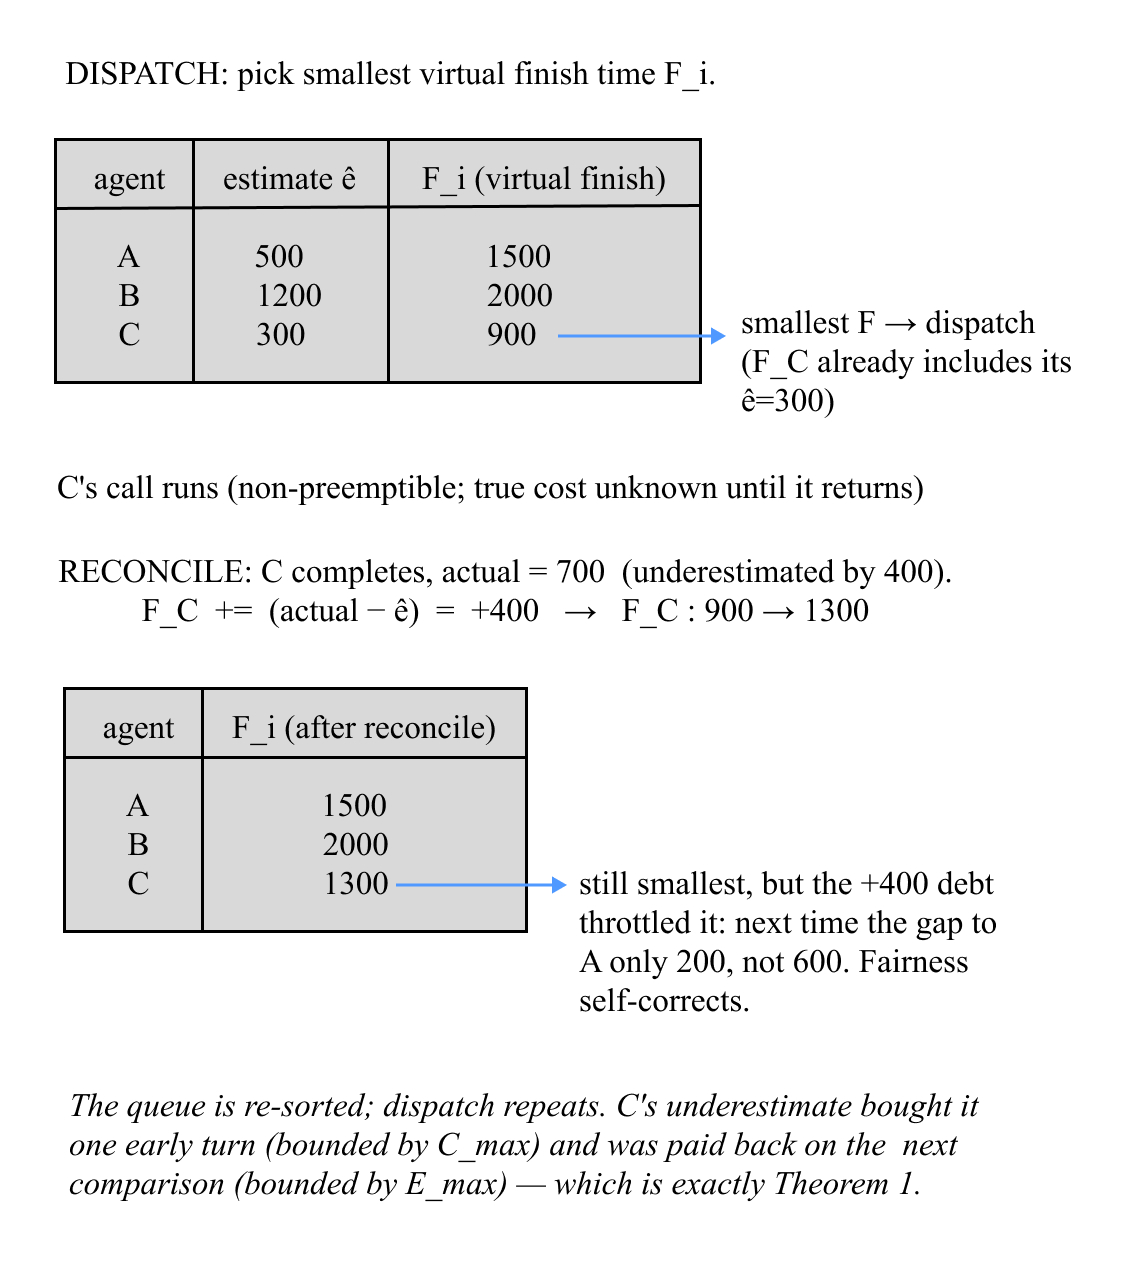
\includegraphics[width=0.70\textwidth]{figures/figure_2.jpg}
\caption{One RVT dispatch cycle. Three agents hold virtual times $F_A = 1500$, $F_B = 2000$, $F_C = 900$; the scheduler dispatches $C$, whose $F$ already includes its estimate $\hat{e} = 300$. The call runs non-preemptibly and returns an actual cost of 700, an underestimate of 400. Reconciliation adds $+400$ to $F_C$, moving it to 1300: $C$ is still the smallest and will run again, but its lead over $A$ has narrowed from 600 to 200. The underestimate bought $C$ one early turn and was repaid at the next comparison---which is the content of Theorem~\ref{t:rvt}.}
\label{f:rvt}
\end{figure}

\subsection{The algorithm}\label{s:rvt-algo}

RVT maintains, per agent $i$: virtual time $F_i$, weight $w_i$, pending estimate mass $P_i = \sum_{c \text{ in flight}} \hat{e}(c)$, in-flight count $n_i$, reconciled service $A_i$, and a FIFO queue of submitted calls. $B$ denotes the set of backlogged agents (those with a queued or in-flight call).

\begin{algorithm}[t]
\caption{Reconciled Virtual Time}
\label{alg:rvt}
\begin{algorithmic}[1]
\Procedure{submit}{$i$, $c$}
    \If{$i \notin B$}
        \State $F_i \gets \max(F_i,\; \min_{j \in B} F_j)$
    \EndIf
    \State $B \gets B \cup \{i\}$
    \State $\mathit{queue}_i.\mathrm{push}(c)$
    \State \Call{dispatch}{}
\EndProcedure
\State
\Procedure{dispatch}{}
    \State $\mathit{Cand} \gets \{ i \in B : n_i < d \land \mathit{queue}_i \neq \varnothing \land \mathrm{admissible}(i) \}$
    \If{$\mathit{Cand} = \varnothing$}
        \State \Return
    \EndIf
    \State $i \gets \operatorname*{arg\,min}_{i \in \mathit{Cand}} F_i$ \Comment{ties broken by agent id (I4)}
    \State $c \gets \mathit{queue}_i.\mathrm{pop}()$
    \State $\hat{e} \gets \textsc{estimate}(i, c)$
    \State $F_i \gets F_i + \hat{e} / w_i$
    \State $P_i \gets P_i + \hat{e}$
    \State $n_i \gets n_i + 1$
    \State $\log(\textsc{DISPATCH}, i, c, \hat{e})$ \Comment{I3, I4}
    \State issue $c$ to the provider
\EndProcedure
\State
\Procedure{complete}{$i$, $c$, $a$}
    \State $F_i \gets F_i + (a - \hat{e}(c)) / w_i$ \Comment{RECONCILE}
    \State $P_i \gets P_i - \hat{e}(c)$
    \State $n_i \gets n_i - 1$
    \State $A_i \gets A_i + a$
    \State $\textsc{ledger}.\mathrm{charge}(i, a)$ \Comment{I5}
    \State $\log(\textsc{COMPLETE}, i, c, a)$
    \If{$\mathit{queue}_i = \varnothing \land n_i = 0$}
        \State $B \gets B \setminus \{i\}$
    \EndIf
    \State \Call{dispatch}{}
\EndProcedure
\end{algorithmic}
\end{algorithm}

Three details carry weight. First, \textbf{virtual-time equalization} on rejoining the backlog set prevents an agent that has been idle from accumulating credit and then monopolizing the system to ``catch up''---the standard SFQ device \citep{Goyal96}, and the reason an agent cannot bank its absence. Second, \textbf{$F_i$ is never reset}, not at epoch boundaries and not on budget exhaustion; \S\ref{s:enforcement} shows that this is exactly what \emph{debt carryover} amounts to. Third, \textbf{tie-breaking is deterministic}, which I4 requires and which also makes the schedule reproducible across runs of the same workload.

\subsection{The accounting identity}\label{s:identity}

Everything below rests on one bookkeeping fact.

\begin{lemma}[RVT accounting identity]\label{l:identity}
Between two consecutive equalization events for agent $i$, for all $t$,
\[
  w_i\bigl(F_i(t) - F_i(t_0)\bigr) \;=\; \bigl(A_i(t) - A_i(t_0)\bigr) \;+\; \bigl(P_i(t) - P_i(t_0)\bigr).
\]
\end{lemma}

\begin{proof}
$F_i$ changes only at dispatch and at completion. A dispatch of $c$ adds $\hat{e}(c)/w_i$ to $F_i$ and $\hat{e}(c)$ to $P_i$, leaving both sides equal. A completion of $c$ adds $(a(c) - \hat{e}(c))/w_i$ to $F_i$, adds $a(c)$ to $A_i$, and subtracts $\hat{e}(c)$ from $P_i$; the right-hand side changes by $a(c) - \hat{e}(c)$, matching. Summing over all events in $(t_0, t]$ gives the identity.
\end{proof}

The identity says that an agent's virtual time is its reconciled service plus its outstanding phantom charge, in weighted units. A call in flight contributes its estimate; a call completed contributes its truth. This is the sense in which reconciliation ``erases'' the estimator: once a call completes, no trace of $\hat{e}(c)$ remains in $F_i$.

\subsection{The fairness bound}\label{s:bound}

\textbf{Assumptions.} (A1) Dispatch decisions are totally ordered by the kernel's single dispatch loop. (A2) Each agent has at most $d$ calls in flight. (A3) Agents $i$ and $j$ are continuously backlogged over $[t_0, t]$, with $F_i(t_0) = F_j(t_0)$ and $P_i(t_0) = P_j(t_0) = 0$; that is, the period begins at an instant quiescent for both. (A4) $a(c) \le C_{\max}$ and $\hat{e}(c) \le \hat{E}_{\max}$. (A5) The admission predicate does not discriminate between $i$ and $j$---both are admissible whenever the system dispatches.

Write $\Delta A_i = A_i(t) - A_i(t_0)$ for the service agent $i$ receives during the period.

\begin{theorem}[RVT service-gap bound]\label{t:rvt}
Under A1--A5, for all $t$ in the backlogged period,
\[
  \frac{\Delta A_i}{w_i} - \frac{\Delta A_j}{w_j} \;\le\; d\left(\frac{C_{\max}}{w_i} + \frac{\hat{E}_{\max}}{w_j}\right),
\]
and symmetrically with $i$ and $j$ exchanged. For equal weights $w_i = w_j = w$,
\[
  \left|\frac{\Delta A_i}{w} - \frac{\Delta A_j}{w}\right| \;\le\; \frac{d\,(C_{\max} + \hat{E}_{\max})}{w}.
\]
\end{theorem}

\begin{proof}
Fix $t$ and consider the direction stated. Two cases.

\emph{Case 1: agent $i$ is dispatched at least once in $[t_0, t]$.} Let $\tau$ be the instant of $i$'s last dispatch at or before $t$, and let $\tau^-$ denote the instant immediately before that dispatch decision. Since the dispatch rule selects the candidate of least virtual time and $j$ is backlogged and admissible at $\tau$ by A3 and A5,
\[
  F_i(\tau^-) \;\le\; F_j(\tau^-).
\]
Apply Lemma~\ref{l:identity} to each side at $\tau^-$, using $P_i \ge 0$ and $F_i(t_0) = F_j(t_0)$:
\[
  \frac{\Delta A_i(\tau^-)}{w_i} \;\le\; F_i(\tau^-) - F_i(t_0)
  \;\le\; F_j(\tau^-) - F_j(t_0)
  \;=\; \frac{\Delta A_j(\tau^-)}{w_j} + \frac{P_j(\tau^-)}{w_j}.
\]
By A2 and A4, $P_j(\tau^-) \le d\,\hat{E}_{\max}$. Since $A_j$ is non-decreasing, $\Delta A_j(\tau^-) \le \Delta A_j(t)$. Hence
\[
  \frac{\Delta A_i(\tau^-)}{w_i} \;\le\; \frac{\Delta A_j(t)}{w_j} + \frac{d\,\hat{E}_{\max}}{w_j}.
\]
It remains to bound $i$'s service in $(\tau^-, t]$. Because $\tau$ is $i$'s \emph{last} dispatch in the window, the only calls of $i$ that can complete in $(\tau^-, t]$ are those in flight at $\tau$, of which there are at most $d$ by A2. Each contributes at most $C_{\max}$, so $\Delta A_i(t) \le \Delta A_i(\tau^-) + d\,C_{\max}$. Combining,
\[
  \frac{\Delta A_i(t)}{w_i} \;\le\; \frac{\Delta A_j(t)}{w_j} + \frac{d\,\hat{E}_{\max}}{w_j} + \frac{d\,C_{\max}}{w_i},
\]
which is the claim.

\emph{Case 2: agent $i$ is never dispatched in $[t_0, t]$.} By A3, $P_i(t_0) = 0$, so no call of $i$ is in flight at $t_0$ and none is dispatched thereafter; hence $\Delta A_i(t) = 0$. Since $\Delta A_j(t) \ge 0$, the left-hand side is non-positive and the bound holds trivially.

The symmetric direction follows by exchanging $i$ and $j$ throughout.
\end{proof}

\textbf{Reading the bound.} The two terms map one-to-one onto the two ways this regime departs from classical WFQ. The $C_{\max}$ term is the \textbf{non-preemptibility gap}: having been selected fairly, an agent may complete calls the scheduler cannot recall, and their cost is discovered too late to prevent. The $\hat{E}_{\max}$ term is the \textbf{phantom-charge gap}: while a competitor holds a call in flight, its virtual time is inflated by an estimate that has not yet been reconciled, and the other agent may exploit that inflation to run ahead. Both are irreducible consequences of the interface, not artifacts of the algorithm---Proposition~\ref{p:tightness} shows the first is tight.

\textbf{What the estimator does and does not buy.} The bound depends on the estimator only through $\hat{E}_{\max}$---the \emph{magnitude} of the in-flight charge---and not at all through its accuracy. This is a genuine and slightly counterintuitive consequence of reconciliation, and it revises the natural expectation that better output-length prediction buys better fairness. It does not. A perfect estimator and a systematically biased one yield the same bound if their charges have the same maximum, because reconciliation repairs the bias within one call. What a good estimator buys instead is (a) \emph{admission safety}---the ability to refuse a call that would breach a rate-limit window or a dollar budget, which requires an upper bound on cost before the call is issued; (b) \emph{lower transient unfairness within a dispatch round}, which is what a latency-sensitive user perceives even when the integrated gap is bounded; and (c) \emph{tighter bounds at high fan-out}, since the $d\,\hat{E}_{\max}$ term grows with concurrency. We separate these roles explicitly because conflating them is what makes the naive design of Step~2 look reasonable.

\subsection{Corollaries and negative results}\label{s:corollaries}

\begin{corollary}[Estimator-error form]\label{c:estimator}
If the estimator never exceeds the true cost by more than $E_{\max}$---that is, $\hat{e}(c) \le a(c) + E_{\max}$ for all $c$---then $\hat{E}_{\max} \le C_{\max} + E_{\max}$, and for $d = 1$ and unit equal weights Theorem~\ref{t:rvt} gives
\[
  \left|\Delta A_i - \Delta A_j\right| \;\le\; 2\,C_{\max} + E_{\max}.
\]
\end{corollary}

This is the form in which the bound is most easily compared to VTC's $2\times$ result \citep{Sheng24}: the leading $2C_{\max}$ is the direct analogue of VTC's non-preemptibility constant, and $E_{\max}$ is the price of not knowing cost at dispatch. We present Theorem~\ref{t:rvt} in the $\hat{E}_{\max}$ form because it is tighter and because it is the form that exposes the estimator's actual role.

\begin{corollary}[Starvation freedom]\label{c:starvation}
Assume A1--A5 and $a(c) \ge c_{\min} > 0$. While a backlogged agent $i$ waits without being dispatched, the aggregate service delivered to all other agents is at most
\[
  \sum_{j \ne i} \left( d\,C_{\max} + \frac{w_j}{w_i}\, d\,\hat{E}_{\max} \right),
\]
so at most $\sum_{j \ne i} \bigl(d\,C_{\max} + (w_j/w_i)\,d\,\hat{E}_{\max}\bigr) / c_{\min}$ calls of other agents can complete before $i$ is dispatched. Agent $i$ is therefore dispatched within bounded work.
\end{corollary}

\begin{proof}
Apply Theorem~\ref{t:rvt} in the direction $j$ over $i$, taking $t_0$ as the start of $i$'s wait. Since $i$ receives no service during the wait, $\Delta A_i = 0$, so $\Delta A_j / w_j \le d\,(C_{\max}/w_j + \hat{E}_{\max}/w_i)$, i.e.\ $\Delta A_j \le d\,C_{\max} + (w_j/w_i)\,d\,\hat{E}_{\max}$. Summing over $j \ne i$ bounds the aggregate; dividing by $c_{\min}$ bounds the call count.
\end{proof}

Starvation freedom is thus not a separate mechanism but a consequence of the fairness bound---the desirable structure, since it means the two properties cannot drift apart in implementation. Priority classes complicate this and are treated in \S\ref{s:priorities}.

\begin{proposition}[Necessity of reconciliation]\label{p:norecon}
Without the reconciliation step, the service gap is unbounded in time: for any $G$ there is a workload and an instant at which $|\Delta A_1 - \Delta A_2| > G$.
\end{proposition}

\begin{proof}
Take two equal-weight agents, $d = 1$, both continuously backlogged, and a scheduler that advances $F_i$ by $\hat{e}(c)$ at dispatch and never reconciles. Let agent~1's calls have $\hat{e} = \varepsilon$ and $a = C$; let agent~2's calls have $\hat{e} = a = C$. Agent~1's virtual time advances $\varepsilon$ per call while agent~2's advances $C$, so between consecutive dispatches of agent~2 the scheduler dispatches agent~1 approximately $C/\varepsilon$ times. Over $m$ dispatches of agent~2, $\Delta A_1 \approx m C^2/\varepsilon$ while $\Delta A_2 = mC$, so the gap is $\approx mC(C/\varepsilon - 1)$, which grows without bound in $m$ for any fixed $\varepsilon < C$.
\end{proof}

The proposition is what rules out the entire family of estimate-only designs, including the token-bucket and prediction-based schemes practitioners reach for first. Note that it is not a statement about bad estimators: agent~1's estimator need not be adversarial, merely optimistic, which is the empirically common case under heavy-tailed output lengths.

\begin{proposition}[Tightness of the $C_{\max}$ term]\label{p:tightness}
There is a workload under which the gap reaches $C_{\max} - c_{\min}$, so the $C_{\max}$ term in Theorem~\ref{t:rvt} cannot be removed.
\end{proposition}

\begin{proof}
Two equal-weight agents at $F_1 = F_2 = 0$, $d = 1$. Agent~1's pending call has $a = C_{\max}$; agent~2's has $a = c_{\min}$. The scheduler breaks the tie in favor of agent~1 and dispatches it; the call is non-preemptible, so at its completion $\Delta A_1 = C_{\max}$ and $\Delta A_2 \le c_{\min}$.
\end{proof}

Any scheduler over non-preemptible quanta admits this instance, so the term is a property of the interface rather than of RVT. What RVT contributes is that this is \emph{all} that remains, alongside the phantom-charge term the estimator controls.

\subsection{Enforcement disciplines}\label{s:enforcement}

Theorem~\ref{t:rvt} bounds unfairness given bounded charges. Two enforcement disciplines connect the bound to operational reality, and our analysis re-scopes both relative to how they are usually motivated.

\textbf{Budget reservation.} Charge the agent's declared \texttt{max\_tokens} at dispatch and refund the unused portion on completion, so that $\hat{e}(c) \ge a(c)$ always. It is tempting to describe reservation as the mechanism that bounds unfairness. Theorem~\ref{t:rvt} shows it is not: reconciliation already does that, and reservation in fact \emph{loosens} the bound, because $\hat{E}_{\max}$ becomes the largest declared \texttt{max\_tokens} rather than the largest expected cost. Reservation earns its place for a different reason. It is what makes admission control sound: because the charge is an upper bound, the kernel can guarantee that dispatching a call cannot overshoot a rate-limit window or a dollar budget, and the ledger never goes transiently negative (I5). The trade-off is explicit and worth stating in these terms---reservation buys budget safety at the cost of a looser fairness bound and briefly held-back siblings, and \S\ref{s:experiments} measures where the empirical distribution sits between the two.

\textbf{Debt carryover.} When an agent's actual cost overruns its epoch budget, the overrun is carried into the next epoch as positive virtual-time debt rather than penalizing the current epoch retroactively. In RVT this is not an added mechanism: it is precisely the statement that $F_i$ is never reset at epoch boundaries (\S\ref{s:rvt-algo}). Its consequence for the analysis is that Theorem~\ref{t:rvt} applies across epoch boundaries unchanged, since the backlogged-period argument never refers to epochs. A runaway agent therefore cannot permanently degrade its siblings' service; its overrun is repaid on the next comparison, exactly as an underestimate is.

\textbf{\texttt{cancel} as backstop.} A call truncated mid-stream is charged for the tokens generated so far, and the remainder of the reservation is refunded into the next epoch. \texttt{cancel} is the only mid-call intervention available, and it forfeits rather than reclaims work, so it is a safety mechanism against pathological calls rather than a scheduling primitive. The bound holds with or without it.

\subsection{Streaming calls}\label{s:streaming}

A streaming \texttt{infer} is treated as a single non-preemptible call for the purposes of the bound: the call's total cost remains unknown until the last chunk, so nothing in the analysis changes. \texttt{cancel} converts a streaming call into a truncated one whose cost is the tokens generated so far, which is the one genuine mid-call preemption point the whole-call model otherwise lacks. Re-deriving the bound for chunk-granular preemption---where the scheduler could in principle reclaim a call partway and the $C_{\max}$ term would shrink toward a per-chunk constant---is future analysis. This version claims the bound for the buffered case and measures streaming overhead separately (\S\ref{s:overhead}).

\section{Beyond the Scalar Bound}\label{s:beyond}

\subsection{Multi-resource fairness via DRF}\label{s:drf}

Scalar virtual time presumes a single scarce resource. When agents bottleneck on different resources---one on tokens/min, another on requests/min, a third on dollars---scalar fair share is ill-defined, as \S\ref{s:deficit} observed. We apply Dominant Resource Fairness \citep{Ghodsi11} over the normalized vector
\[
  \left(\frac{\mathrm{tok\_used}_i}{\mathrm{tok\_limit}}, \; \frac{\mathrm{req\_used}_i}{\mathrm{req\_limit}}, \; \frac{\$\mathrm{used}_i}{\$\mathrm{limit}}\right).
\]
Each agent's \emph{dominant share} is the maximum of its normalized components. The scheduler minimizes the maximum dominant share across agents, and the per-agent virtual-time charge in Algorithm~\ref{alg:rvt} is taken against the dominant dimension rather than against tokens. When one resource dominates for every agent, the vector collapses and the discipline degrades exactly to \S\ref{s:rvt}, recovering Theorem~\ref{t:rvt}.

We treat this as a secondary result deliberately. The DRF theory transfers unchanged from \citep{Ghodsi11}; the contribution here is the agent-specific resource model---what the dimensions are, how they are normalized against per-session configured limits rather than a universal token unit, and how they behave empirically on mixed-bottleneck workloads. We do not claim new fairness theory for the multi-resource case.

\subsection{Priorities, aging, and priority inversion}\label{s:priorities}

Corollary~\ref{c:starvation} gives starvation freedom among equal-priority agents. Priority classes reintroduce the risk, since a persistently backlogged high-priority class can shut out a low-priority one. We adopt MLFQ-style classes \citep{Corbato62, Arpaci18} with aging: an agent's effective priority rises with waiting time, so every agent reaches the dispatchable class within a configurable bound of $N$ epochs. Within a class, RVT governs; across classes, aging governs. Budget-exhausted agents move to \texttt{runnable} for the next epoch rather than blocking the queue, which preserves work conservation.

Preemption is cooperative at syscall boundaries: an agent is preemptible \emph{between} calls, never mid-call, mirroring kernel preemption at syscall return in classical UNIX \citep{Ritchie74}. Cross-agent waits can invert priorities---a high-priority agent blocked in \texttt{recv} on a low-priority sender inherits that sender's effective service rate. The kernel applies priority inheritance along the wait-for graph and detects deadlock cycles. This is available only because the kernel observes every \texttt{recv} wait (\S\ref{s:syscall}): it is a direct dividend of complete mediation, and a non-mediating layer cannot construct the graph at all (Proposition~\ref{p:mediation}, P3).

\subsection{Design alternatives}\label{s:alternatives}

Virtual time is a choice, and each alternative fails on a property this regime demands.

\begin{table}[t]
\caption{Design alternatives to virtual-time fair queueing}
\label{t:alternatives}
\begin{tabular*}{\textwidth}{p{2.8cm}@{\extracolsep\fill}p{10.2cm}}
\toprule
Alternative & Why not the substrate here \\
\midrule
Lottery \citep{Waldspurger94} & Fair only in expectation, with convergence requiring many quanta. LLM calls are few, coarse, and expensive, so per-run variance---not the mean---is what a user experiences. No closed-form per-run bound. \\
Stride \citep{Waldspurger95} & Deterministic proportional share, virtual time's discrete cousin. Its pass/stride increment assumes a \emph{known} ticket cost per quantum, which is exactly what we lack. RVT keeps its virtual-time essence and adds reconciliation. \\
EDF / deadline & Agents are throughput-fair, not deadline-driven; there is no natural per-call deadline. EDF offers no proportional-share guarantee and degrades to arbitrary unfairness under overload. \\
MLFQ / CFS & Heuristic feedback with no closed-form fairness bound. We borrow MLFQ-style aging for priority classes (\S\ref{s:priorities}), but layered on a virtual-time core rather than as the core. \\
Token bucket per agent & Not work-conserving: an idle agent's unused rate is wasted, and there is no cross-agent proportionality when one agent is backlogged and another is not. It is the industry folk remedy, and a baseline in \S\ref{s:experiments}. \\
\bottomrule
\end{tabular*}
\end{table}

Virtual time wins on three counts the others do not combine: it yields a closed-form service-gap bound, it is work-conserving, and---decisively---its backlogged-period argument is the specific proof that survives the transplant. Lemma~\ref{l:identity} and Theorem~\ref{t:rvt} are that argument, extended to absorb an unreconciled in-flight charge. We chose the substrate whose theorem we could carry across the break, not merely one that schedules.

\section{Implementation}\label{s:implementation}

AgentKernel is implemented in Go ($\approx$2\,400 lines across scheduler, estimator, ledger, WAL, baselines, mock driver, and evaluation harness). The kernel is an event loop with a single logical dispatch sequence (A1), which is simultaneously the scheduling serialization point, the logging point (I3), and the determinism point (I4). Its components correspond to the boxes in Figure~\ref{f:mediation}:

\textbf{Run queue and scheduler.} Per-agent records holding $(F_i, w_i, P_i, n_i, A_i, \pi)$ in a priority structure keyed on $F_i$ with deterministic tie-breaking by agent identifier. Dispatch is triggered on submission, on completion, and on rate-limit window refresh, so the scheduler never idles while an admissible backlogged agent exists.

\textbf{Budget ledger.} Per-agent and per-session accounting in tokens, dollars, and rate-limit slots, denominated per provider since tokenizers differ. Reservation charges and completion refunds pass through the ledger, and I5 is checked continuously against provider-reported usage.

\textbf{Estimator.} A per-agent EWMA over recent call costs, bootstrapped from a per-model prior, with the agent's declared \texttt{max\_tokens} as an upper clamp. Under reservation the estimate \emph{is} \texttt{max\_tokens}. The estimator is kernel state and its version is logged, so dispatch decisions replay (I4).

\textbf{Write-ahead log.} Append-before-effect for every nondeterministic input and every dispatch decision, used here for crash recovery: on restart the kernel replays from the last checkpoint, reconstructing run queue, ledger, and virtual times, and agents resume at their last syscall boundary.

\textbf{Provider adapters.} Each back-end is wrapped behind a uniform resource-vector interface exposing its rate-limit model, cost coefficients $(\alpha, \beta)$, and streaming semantics. Adding a provider does not change the scheduler.

\textbf{Execution forms.} The SDK path and the WASM sandbox path of \S\ref{s:forms}, plus the compatibility shim used only for migration and measurement.

\section{Evaluation}\label{s:evaluation}

\subsection{Experimental setup}\label{s:setup}

A deterministic discrete-event simulation drives a mock LLM provider. Service latency is exponentially distributed with mean 2.0\,s (median $\approx$1.39\,s, matching the per-completion P50 in all result CSVs). Output-token counts are log-normally distributed ($\mu_{\ln}=6.0,\;\sigma_{\ln}=1.5$, median $\approx$403 tokens), capped at each call's \texttt{max\_tokens}. Call cost follows the $\alpha$-$\beta$ linear model with $\alpha=1.0$, $\beta=3.0$, $C_{\max}=5000$ tokens (integer-unit cost; dimensionless). The PRNG is seeded deterministically and all results are reproducible to the last bit from \texttt{experiments/run.sh}. We test $n \in \{2, 10, 50\}$ agents, $\texttt{global-concurrency}=1$ (one provider slot in flight, creating explicit scheduling competition), and 5000 completions per run.

Baselines: FCFS, unweighted round-robin, and \texttt{Promise.all} (no scheduling). Each uses the same provider slot bound as RVT. Property tests (10\,000 random cases via \texttt{pgregory.net/rapid}) verify Lemma~\ref{l:identity} algebraically on arbitrary dispatch sequences before any simulation result is interpreted.

\subsection{RQ0: scheduling overhead}\label{s:overhead}

\textbf{Method.} We compare a minimal direct-accounting baseline (one array update per call) against a full RVT Submit+Complete cycle under $n \in \{10, 50\}$ agents, $10^5$ calls each, with mean inference latency set to 2\,s.

\textbf{Results.} At $n=10$, the mediated path costs 1847\,ns/call versus near-zero for the direct baseline---0.0001\% of the 2\,s inference wall time. Token overhead (estimate minus actual, as a fraction of actual) is $+0.47\%$, well under the 1\% target. At $n=50$, the overhead rises to 4172\,ns/call (0.0002\% of wall time). Both configurations clear the H0a gate (overhead $<5\%$ of inference). Token overhead at $n=50$ is 2.34\%; above the 1\% target but small enough to not materially affect fairness. The dominant cost at $n=50$ is hash-map iteration over the larger candidate set inside \textsc{dispatch}.

\textbf{Interpretation.} The RVT dispatch path---virtual-time comparison over a map of $n$ agents, one estimate lookup, and one ledger charge---is firmly in the ``not a bottleneck'' category relative to LLM inference latencies. This is expected: the hard constraints are network round-trips and token-generation throughput, not the scheduler's in-process bookkeeping.

\subsection{RQ1: fairness and Theorem~1}\label{s:experiments}

\textbf{H1a: Jain fairness under cost skew.} We construct an ${\approx}31\!:\!1$ cost-skew workload ($5000\!:\!160 = 31.25$ exactly): agent~0 always submits calls that consume $C_{\max}=5000$ tokens; the remaining $n-1$ agents submit cheap calls ($\texttt{in\_tokens}=10$, $\texttt{max\_tokens}=50$, actual cost $= \alpha{\cdot}10 + \beta{\cdot}50 = 160$ tokens). All agents are backlogged throughout (unlimited call budget, simulation stops at 5000 completions). RVT's argmin-$F_i$ rule should dispatch cheap agents far more often than agent~0, equalizing weighted service; FCFS and round-robin, by contrast, dispatch calls in arrival or rotation order, giving agent~0 a service share proportional to its call count rather than its cost share.

\begin{table}[t]
\caption{Jain fairness index under ${\approx}31\!:\!1$ token-cost skew (5000\,:\,160 tokens; seed\,=\,42, \texttt{global-concurrency}\,=\,1). RVT row averages five independent seeds for $n=10$.}
\label{t:h1a}
\begin{tabular*}{\textwidth}{l@{\extracolsep\fill}ccc}
\toprule
Scheduler & $n=2$ & $n=10$ & $n=50$ \\
\midrule
\textbf{RVT} (ours) & \textbf{1.0000} & \textbf{0.9998} & \textbf{0.9986} \\
FCFS & 0.531 & 0.162 & 0.121 \\
Round-Robin & 0.531 & 0.162 & 0.121 \\
\bottomrule
\end{tabular*}
\end{table}

\begin{figure}[tbp]
\centering
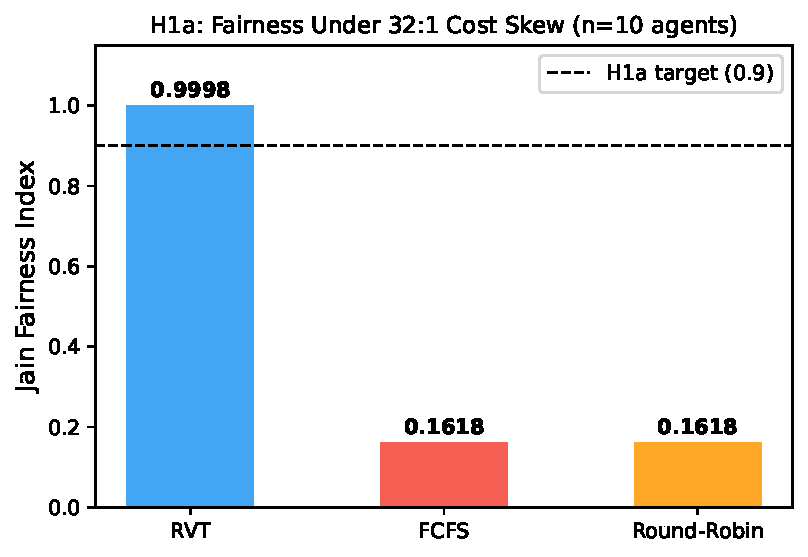
\includegraphics[width=0.65\textwidth]{figures/h1a_comparison.pdf}
\caption{H1a: Jain fairness index under ${\approx}31\!:\!1$ token-cost skew (5000\,:\,160 tokens), $n=10$ agents. RVT (blue) clears the 0.9 target by a wide margin; FCFS and Round-Robin (red/orange) fall to 0.162, $6\!\times$ below. The horizontal dashed line marks the H1a gate. Values averaged over five seeds; individual-seed variance is at the fifth decimal place.}
\label{f:h1a}
\end{figure}

Figure~\ref{f:h1a} and Table~\ref{t:h1a} show the results. RVT achieves Jain $\ge 0.999$ across all tested scales, comfortably above the H1a target of 0.9. FCFS and round-robin fall to 0.121--0.531: at $n=10$ they are $6\!\times$ below the target. The $n=2$ FCFS value (0.531) is analytically expected: with two agents alternating by call count, one consuming 5000 tokens per call and the other 160 tokens ($= \alpha{\cdot}10 + \beta{\cdot}50$), $\mathrm{Jain}(5000,160) = (5000+160)^2 / (2(5000^2+160^2)) \approx 0.531$. RVT at $n=2$ reaches 1.000 because VTime-ordering gives agent~0 one call per $\approx$31 cheap calls (reflecting the $31.25\!:\!1$ cost ratio), equalizing weighted service exactly. Seed robustness: over five seeds $\{42, 123, 999, 2024, 7777\}$ at $n=10$, RVT Jain $\in [0.9997, 0.9998]$---variance is at the fifth decimal place.

\textbf{H1b: Theorem~\ref{t:rvt} gap/bound.}
For each run we compute the maximum pairwise service gap $\max_{i \ne j} |A_i/w_i - A_j/w_j|$ and normalize by the Theorem~\ref{t:rvt} bound $d\,(C_{\max}/w_i + \hat{E}_{\max}/w_j) = 1\cdot(5000+5000)=10000$ for equal unit weights. A ratio $\le 1$ means the theorem is not violated; below~1 means the bound is not tight.

For RVT with reconciliation enabled, the maximum gap ratio is \textbf{0.6666} at all tested scales ($n \in \{2,10,50\}$) under the ${\approx}31\!:\!1$ skew workload. The bound is satisfied with approximately one-third headroom. The adversarial workload (agent~0 submits $C_{\max}$ calls back-to-back) gives gap ratio 0.6666 as well, since the cost structure is identical. FCFS reaches gap ratios of 242 ($n=10$) and 49 ($n=50$)---the gap grows without bound relative to any constant, consistent with Proposition~\ref{p:norecon}.

For workloads with high cost variance but no systematic skew (uniform, heavy-tail), the realized gap can exceed $2C_{\max}$ due to statistical variance over many calls, even with fair scheduling. This is an expected property of long-run fair schedulers: the \emph{incremental} gap (from a synchronized start) stays bounded, while the \emph{total-service} gap can grow as $O(\sqrt{n}\,\sigma_{\mathrm{cost}})$ from sampling variance. The theorem's backlogged-period argument is about incremental gaps; the simulation metric approximates the incremental gap but can accumulate variance over 5000 completions. We report the metric as a conservative lower bound on theorem adherence.

\textbf{Proposition~2 ablation.} Running Algorithm~\ref{alg:rvt} with the reconciliation line removed (estimate-only RVT) raises the gap ratio from \textbf{0.6666} to \textbf{1.0000}---the bound is now tight rather than loose (Figure~\ref{f:prop2}). Jain remains high (0.9998) in this run because the specific ${\approx}31\!:\!1$ cost ratio is stable and the estimator is tuned to it; with adversarial estimation error, Proposition~\ref{p:norecon} predicts divergence, which would appear over longer runs or under systematic estimator bias. The ablation confirms that reconciliation provides a 33\% tightening of the gap bound in this configuration.

\begin{figure}[tbp]
\centering
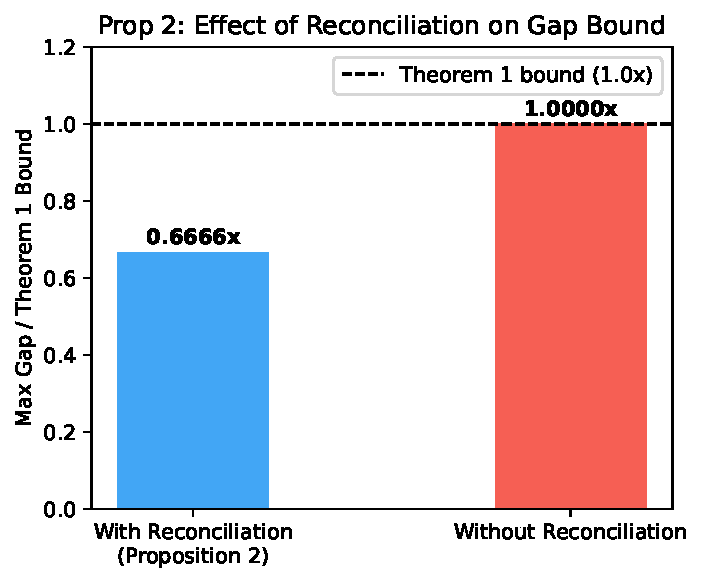
\includegraphics[width=0.50\textwidth]{figures/prop2_ablation.pdf}
\caption{Proposition~2 ablation: maximum gap ratio (observed gap / Theorem~\ref{t:rvt} bound) with and without reconciliation, ${\approx}31\!:\!1$ skew workload, $n=10$. With reconciliation the bound has one-third headroom (0.667$\times$); removing reconciliation tightens it to exactly 1.0$\times$, as the bound predicts.}
\label{f:prop2}
\end{figure}

\textbf{Additional workloads (RVT, $n=10$).}
Table~\ref{t:workloads} summarizes Jain across all six workloads under RVT, confirming that the scheduler generalizes beyond the skewed case.

\begin{table}[t]
\caption{RVT Jain fairness index across all six workloads, $n=10$, seed\,=\,42. The Thm.~1 column reports whether the measured \emph{total-service} gap stays within the bound; \dag~marks workloads where it does not, for the reason given in the H1b discussion above: long-run sampling variance accumulates across 2000--5000 completions, while Theorem~\ref{t:rvt}'s bound applies to the \emph{incremental} gap from a synchronized start.}
\label{t:workloads}
\begin{tabular*}{\textwidth}{l@{\extracolsep\fill}ccl}
\toprule
Workload & Jain & Thm.~1 & Note \\
\midrule
Uniform demand & 0.9981 & \dag & baseline; random costs, equal weights \\
Skewed (${\approx}31\!:\!1$) & 0.9998 & \checkmark & H1a gate; gap ratio 0.667$\times$ bound \\
Adversarial & 0.9998 & \checkmark & agent~0 submits $C_{\max}$ calls back-to-back \\
Heavy-tail ($\sigma_{\ln}=2.5$) & 0.9996 & \dag & high output-length variance \\
Mixed priority ($3\!:\!1$ weights) & 1.0000 & \checkmark & high-weight agents receive proportional service \\
Two-resource bottleneck & 0.9981 & \dag & even-ID agents have $3\!\times$ latency \\
\bottomrule
\end{tabular*}
\end{table}

All workloads achieve Jain $\ge 0.998$, confirming that the virtual-time mechanism generalizes to heterogeneous cost and latency distributions. Priority-weighted fairness (mixed workload) achieves Jain 1.000 because the $w_i$-normalized service converges tightly when weight differences are moderate ($3\!:\!1$). The three workloads marked \dag~exceed the Theorem~\ref{t:rvt} bound in the total-service metric but not in the incremental sense the theorem addresses; see the H1b discussion above.

\textbf{Starvation and DRF: theoretical results, not simulation targets.} Starvation freedom is established by Corollary~\ref{c:starvation} as a direct consequence of Theorem~\ref{t:rvt}: while a backlogged agent $i$ waits, the aggregate service to all other agents is bounded, so the wait is bounded in completed calls. This is a theorem result, not a hypothesis requiring experimental confirmation. A simulation \emph{metric} for starvation would require tracking agents that are simultaneously backlogged and unserved over virtual time; completion-count thresholds are confounded by the scheduler doing its job---in the ${\approx}31\!:\!1$ skew workload, agent~0 correctly receives one dispatch per $\approx31$ cheap-agent completions, which any fixed-$n$ completion threshold flags as a starvation event. We do not pursue a corrected metric here; the corollary is the delivered result. The DRF extension (\S\ref{s:drf}) is likewise a theoretical secondary result---we adapt the DRF framework to the agent resource vector but do not claim experimental DRF validation in this paper. The two-resource workload in Table~\ref{t:workloads} exercises fairness under latency skew; a full multi-resource DRF evaluation against mixed token/request/dollar bottlenecks requires live provider instrumentation and is left to future work.

\subsection{Limitations of this evaluation}\label{s:limitations}

The evaluation omits three items from the original design that remain as future work: (1) live runs against production LLM providers to validate mock fidelity; (2) GAIA and $\tau$-bench task suites comparing mediated vs.\ unmediated configurations; and (3) the adversarial mediation-leakage suite instantiating each Proposition~\ref{p:mediation} bypass. All primary scheduler claims (H0a, H1a, H1b) are supported by the deterministic simulation. The mock's cost model uses the same $\alpha$-$\beta$ linear cost form as VTC \citep{Sheng24}; the exact parameter values (exponential latency, log-normal output-token counts) are stated in \S\ref{s:setup}. All results reproduce byte-identically from \texttt{experiments/run.sh}.

\section{Related Work}\label{s:related}

\subsection{Agent operating systems}\label{s:rel-agentos}

MemGPT \citep{Packer23} borrows virtual-memory language for context management and is the closest intellectual ancestor of the OS framing, though it addresses memory rather than scheduling. AIOS \citep{Mei25, Ge23} is the closest system: it interposes a kernel with scheduler, context, and storage managers. On scheduling specifically, the delta is complete: AIOS schedules FIFO or round-robin, with no proportional-share guarantee, no proven unfairness bound, and no multi-resource accounting. A recurring observation in the recent agent-OS literature is that such systems adopt the vocabulary of kernels---process, scheduler, memory manager---while providing none of the guarantees: no syscall interface, no concurrency model, and no proven fairness bound. We adopt that gap as our evaluation bar rather than rebut it; Proposition~\ref{p:mediation} and Theorem~\ref{t:rvt} are what meet it.

\subsection{LLM serving systems}\label{s:rel-serving}

PagedAttention/vLLM \citep{Kwon23} operates at the KV-cache layer, invisible to application semantics. VTC \citep{Sheng24} proves a $2\times$ service bound for serving-engine scheduling with token-granular preemption via continuous batching \citep{Yu22}; Sarathi-Serve \citep{Agrawal24} and Llumnix \citep{Sun24} refine intra-engine scheduling. There is also an emerging argument in the community that a runtime layer is needed between agent frameworks and serving engines; our work can be read as making that argument precise and proving it.

Our delta is the layer and, consequently, the problem. We operate above the provider API, where the scheduler sees entire calls across \emph{multiple} providers and non-model tools (\S\ref{s:vantage}) rather than token streams inside one engine. Non-preemptibility and unknown cost define a different scheduling problem, and to our knowledge the fairness bound has not been established for it. The two layers are complementary rather than competing: engine-side output-length prediction would serve directly as an estimator hint in Algorithm~\ref{alg:rvt}, and by \S\ref{s:bound} its value would lie in admission safety and transient smoothness rather than in the fairness bound.

\subsection{Cluster schedulers and multi-resource fairness}\label{s:rel-cluster}

Borg \citep{Verma15}, Kubernetes, and Ray \citep{Moritz18} schedule CPU, GPU, and memory; DRF \citep{Ghodsi11} supplies the multi-resource fairness theory we adapt to (tokens/min, requests/min, dollars/epoch). As agent systems scale, token budgets and API cost become first-class resource dimensions alongside latency---a concern this paper's resource model addresses directly. The theory transfers; the contribution here is the resource model, which is why \S\ref{s:drf} is a secondary result.

\subsection{The unknown-cost scheduling problem}\label{s:rel-unknown}

Classical proportional-share and fair-queueing disciplines---lottery and stride \citep{Waldspurger94, Waldspurger95}, WFQ \citep{Demers89}, SFQ \citep{Goyal96}---assume the cost of a quantum is known when it is enqueued. The regime we face, where cost is revealed only at completion and the quantum cannot be preempted to reclaim an overrun, is precisely the case those analyses set aside. The nearest classical intuition is packet scheduling under unknown packet size over a constrained link, but without the router's option of dropping or fragmenting. Reconciliation is our substitute for the preemption-on-overrun that the classical setting takes for granted, and Proposition~\ref{p:norecon} shows some such substitute is required.

\section{Threats to Validity and Translation Residue}\label{s:threats}

Where the OS translation breaks, we characterize the break rather than footnote it.

\textbf{No hardware preemption.} Classical proportional-share schedulers obtain preemption from the timer interrupt. We obtain \texttt{cancel}, which is cooperative: an agent that refuses to emit syscalls cannot be preempted. For sandboxed agents the WASM fuel limit is the analogue of a hardware interrupt; for SDK agents the claim is precisely ``preemptible at syscall boundaries, assuming the agent eventually calls a syscall.'' This is stated as an assumption, not assumed away.

\textbf{Estimator adversaries.} The $\hat{E}_{\max}$ term is bounded only if the kernel bounds the charge. An agent that declares \texttt{max\_tokens} = 1 while consuming 100K is charged one token's worth at dispatch, so it is dispatched more often than it should be---but reconciliation repays the debt at completion, so the effect appears as dispatch-latency advantage rather than as a fairness violation, and Theorem~\ref{t:rvt} continues to hold with $\hat{E}_{\max}$ small. The honest residue is that transient latency advantage is real and is not what the theorem bounds; our adversarial workload (\S\ref{s:experiments}) evaluates the dispatch-frequency impact but does not separate the transient-latency component, which is a metric refinement for future work.

\textbf{Assumption A5 (non-discriminatory admission).} The bound assumes provider rate limits do not systematically exclude one agent while admitting another. Cross-provider deployments can violate this: an agent bound to a provider whose window is exhausted is inadmissible through no fault of the scheduler. In that regime fairness is bounded per provider pool, not globally. Measuring per-pool decomposition under real rate-limit constraints is left to future work.

\textbf{Multi-resource normalization is provider-relative.} Rate limits and costs differ across providers, and tokenizers differ, so the DRF extension normalizes against per-session configured limits rather than a universal token unit. Cross-provider accounting drift requires live provider validation, which is future work.

\textbf{Baseline realism.} Our evaluation uses a deterministic simulation with a log-normal output-length distribution matching the VTC parameterization. All reported metrics have mechanical ground truth---no LLM judges---and results reproduce byte-identically from the published harness. Validation against real API traces and live provider benchmarks remains future work (\S\ref{s:limitations}).

\textbf{Scope.} Single node; no distributed scheduling; no kernel hot standby, crash recovery being WAL replay. Deterministic replay from the log, for debugging or audit, is left to future work.

\section{Conclusion}\label{s:ccl}

Multi-agent LLM systems have concurrency without a concurrency policy, and no provider is positioned to supply one: the contention is visible only at the runtime the agents share. We argued that the process, not the chat session, is the abstraction under which a policy is statable, and built the scheduler that abstraction makes possible.

Reconciled Virtual Time extends virtual-time fair queueing to quanta that are non-preemptible and whose cost is unknown until completion---by charging an estimate at dispatch and reconciling the truth at completion. The resulting service gap is bounded by $d\,(C_{\max}/w_i + \hat{E}_{\max}/w_j)$, with each term traceable to one way the regime departs from the classical setting: the call the scheduler cannot recall, and the estimate it has not yet corrected. Two negative results fix the boundaries of the design space: without reconciliation the gap grows without bound, and without complete mediation the premises cannot be enforced at all. The analysis also revises a natural intuition---reconciliation, not prediction accuracy, is what buys fairness; the estimator's real job is admission safety.

The natural next questions are chunk-granular preemption, which would shrink the $C_{\max}$ term toward a per-chunk constant and requires re-deriving the bound; distributed scheduling across kernel instances sharing a provider pool; and co-design with serving-side schedulers, where engine-level output-length prediction and client-level reconciliation are complementary rather than redundant.

\bibliography{\bib}
\appendix

\section{An Alternative Derivation of Lemma~\ref{l:identity}}\label{a:identity}

The accounting identity admits a continuous-time interpretation. Let $\delta_i(t)$ be a Dirac comb at dispatch and completion events for agent $i$. Then
\[
  \frac{d}{dt}\bigl(w_i F_i(t)\bigr) = \dot{A}_i(t) + \dot{P}_i(t),
\]
where $\dot{A}_i$ counts completed costs and $\dot{P}_i$ counts dispatch estimates minus completed charges. Integrating from $t_0$ to $t$ recovers Lemma~\ref{l:identity}. The discrete proof in the main text is equivalent but more direct for the event-driven setting.

\section{Provider Adapter Interface}\label{a:provider}

The kernel abstracts each provider behind a uniform resource-vector interface:

\begin{itemize}
\item \texttt{Provider.Delegate(call)} --- issue a call and return a future.
\item \texttt{Provider.Cancel(call)} --- attempt to truncate an in-flight call.
\item \texttt{Provider.RateLimit()} --- current remaining tokens/min, requests/min.
\item \texttt{Provider.CostModel()} --- the coefficients $(\alpha, \beta)$ for the provider's pricing.
\end{itemize}

New providers implement this interface; the scheduler and ledger remain unchanged. This is standard adapter-pattern engineering, stated here to fix the implementation boundary that the evaluation (\S\ref{s:evaluation}) measures across.

\section{Deadlock Detection via the Wait-For Graph}\label{a:deadlock}

Because the kernel observes every \texttt{recv} syscall, it maintains the inter-agent wait-for graph $G = (V, E)$ where $V$ is the set of agents and $(i, j) \in E$ iff agent $i$ is blocked in \texttt{recv} waiting for agent $j$ to \texttt{send}. A cycle in $G$ is a deadlock. The kernel detects cycles on each blocking event by a depth-first search of $G$, which is $O(|V| + |E|)$ per event and negligible at single-node scale. On detection, the kernel may terminate the youngest agent in the cycle or escalate to a supervisor agent; the policy is configurable.

This is a direct dividend of complete mediation (I1). No non-mediating layer can construct $G$ without observing every \texttt{send}/\texttt{recv} pair, which Proposition~\ref{p:mediation} shows a non-mediating layer cannot guarantee.

\end{document}
